\chapter{基于知识图谱的故障预测}\label{chapter-predict-failure}
在云计算场景中,分布式集群会随时间产生大量的事件序列。根据这些实时事件序列,准确地预测未来会发生的故障始终面临着巨大挑战。已有的方法\cite{pitakrat2018hora,zhang2018prefix,baldoni2015line,xu2016health,cheng2018machine,du2017deeplog,das2018desh,islam2017predicting,cheng2018machine,du2017deeplog,das2018desh,gao2020task}均集中在基于时序数据的故障预测方法,只能预测到是否会发生故障,缺乏可解释性,详细分析如\ref{predict-analysis}所述。

为了解决故障难以准确预知的问题,本章提出了引入知识图谱的故障预测方案。本文的故障预测模型可以预测到会产生何种故障。另外,知识图谱增强了预测结果的可解释性,有助于运维人员分析、调整系统,防止故障真正发生带来损失。本模型在进行故障预测时取得了最高的准确率,且具有更高的细粒度与更好的可解释性。

本章节共分为4小节介绍基于知识图谱的故障预测模型(Fault Prediction with Knowledge Graph,FPKG)。首先,本章介绍了所提故障预测模型的总体框架图。随后,本章进行了场景分析,列出了本文场景中故障预测要解决的问题。然后详细介绍了引入组件-事件知识图谱的故障预测模型。最后,本章在数据集上进行了充分的实验,并对结果进行了详尽分析。
\section{总体框架}
本章所提故障预测方案的总体框架图如\ref{kg-predict-total}所示。由图可见,故障知识库中存储着多个故障类型对应的组件-事件知识图谱,这些知识图谱均是历史数据经过上文所述图谱构建方法得到的。实时数据(日志和指标时序数据)会经过事件生成模块,转化为实时事件序列。实时事件序列输入故障预测模块后,经BiLSTM编码,会与知识库中每个经Attention-RGCN编码的组件-事件知识图谱计算匹配度。训练模块会最大化实时事件序列与对应组件-事件知识图谱的匹配度,并更新模型参数。预测模块会输出匹配度最高的知识图谱作为预测结果,用于检测故障预测模型效果,同时会根据匹配到的知识图谱与实时事件,标出实时事件间的触发关系,解释故障触发过程。
\begin{figure}[htbp]
    \centering
    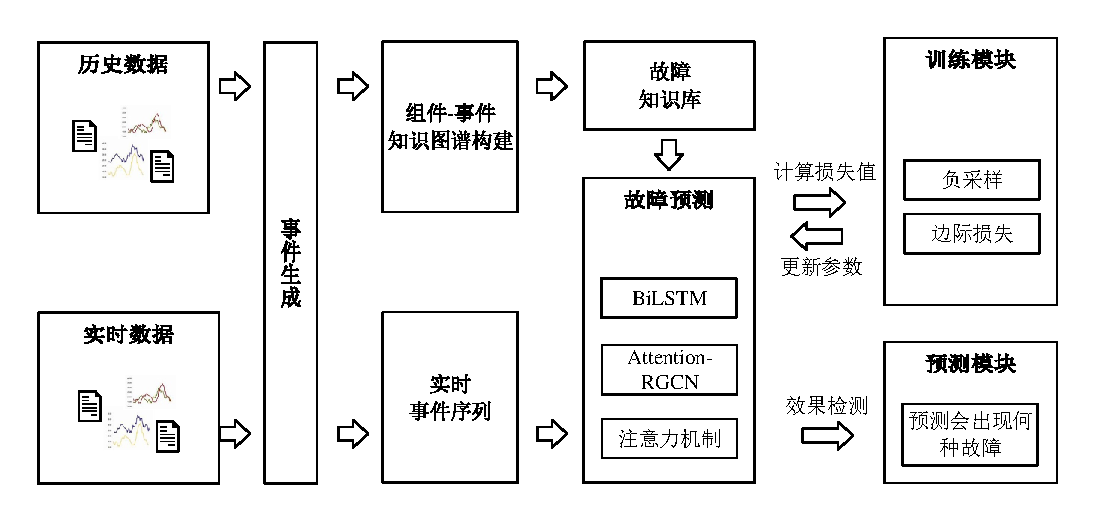
\includegraphics[width=.8\textwidth]{kg-predict-total.pdf}
    \caption{基于事件序列和知识图谱的故障预测总体架构图\label{kg-predict-total}}
\end{figure}
\section{场景分析}\label{predict-analysis}
目前已经存在着较多相关的工作,均集中在基于数据的时序性展开研究。文献\parencite{pitakrat2018hora,zhang2018prefix,baldoni2015line}使用了统计学习和机器学习方法,如隐半马尔可夫模型(Hidden Semi-Markov Model,HSMM)、支持向量机(SVM)。然而,HSMM和SVM都建立于所有输入都是平稳且相互独立的假设之上,这种假设在云计算场景中是不成立的,因为云计算场景中不同组件产生的事件信息之间会存在一定的关联,比如先后时间顺序。为了处理时间序列数据进行故障预测,文献\parencite{xu2016health,cheng2018machine,du2017deeplog,das2018desh,islam2017predicting}使用深度学习方法如循环神经网络(RNN)和长短期记忆神经网络(LSTM)进行预测。但RNN存在着难以克服的缺点,它会遗忘掉较远距离的数据信息。LSTM则克服了这个缺点,可以通过记忆门依然保留长距离数据的信息。文献\parencite{cheng2018machine,du2017deeplog,das2018desh}等工作已经使用LSTM在故障预测任务上比HSMM、SVM和RNN取得了更高的准确率。上述的方法都使用CPU使用率、内存使用率、未映射页缓存、平均磁盘I/O时间和磁盘使用率作为输入,把系统任务是否会失败作为输出。随后,文献\parencite{gao2020task}在LSTM的基础上使用了多层的Bi-LSTM、引入了任务优先级、提交时间、提交次数等更多的特征,还根据不同数据对故障的重要性赋予其不同的权重。

在本文场景中进行故障预测时,除了要分析时序数据外,还需要考虑以下场景特性:

(1)数据形式为事件序列。本文所有的数据,除了包括上文提到的CPU使用率、内存使用率、未映射页缓存、平均磁盘I/O时间和磁盘使用率,另外还有新引入的微服务启动、重启、程序运行日志等数据,都已经被转为统一规范化的事件数据,所以要处理的数据为事件序列。

(2)需引入知识图谱增强可解释性。本文在进行故障预测时,已经存在了前文所构建的组件-事件知识图谱。引入知识图谱会使故障预测结果更具可解释性,还能具体到会出现何种故障。
\begin{figure}[htbp]
    \centering
    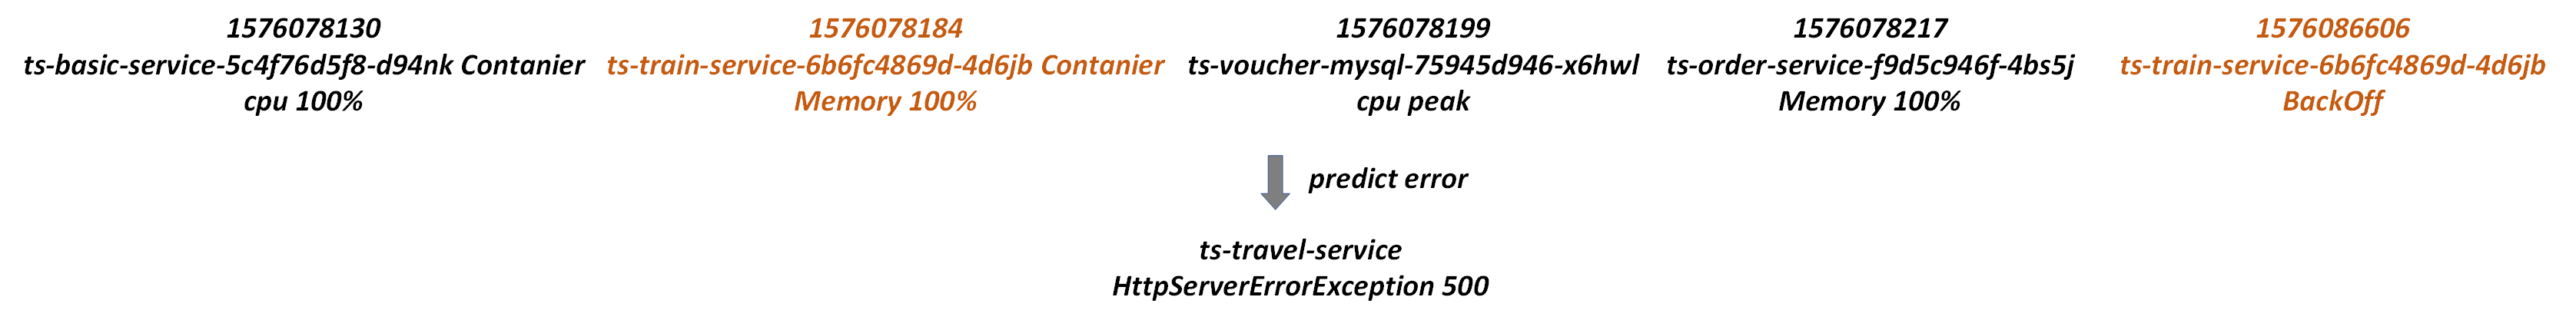
\includegraphics[width=1.0\textwidth]{predict-case.png}
    \caption{事件序列故障预测\label{predict-case}}
\end{figure}

(3)事件权重分配需要考虑序列上下文,不能仅根据数据对故障的重要性赋予权重。如图\ref{predict-case}所示是一个实时事件序列案例。在进行故障预测时,并不是每个异常事件都是同等重要的。$ts-train-service-6b6fc4869d-4d6jb$上的$Contanier Memory 100\%$和$ts-train-service-6b6fc4869d-4d6jb$上的$BackOff$事件应当比其他事件的重要性更高,因为这两个事件的发生意味着$ts-train-service$所在的$Container$已经内存不足,使得$ts-train-service$微服务无法正常启动,后续导致$ts-travel-service$发生$HttpServerErrorException 500$的可能性极高。而其它的事件如$ts-order-service-f9d5c946f-4bs5j$上的$Memory 100\%$虽然对图\ref{order-service-error}的“订票服务不可用”故障较为重要,但是并没有发生后续的关键事件$ts-order-service$上的$BackOff$,所以其重要性较低。

基于以上的分析,本文在编码事件序列时,依然选择基于LSTM的模型,但不同于之前根据每个事件元素对故障重要程度赋予权重\cite{gao2020task},本文选择使用组件-事件知识图谱的嵌入向量来对各个时间单元的数据自适应注意力权重,即由组件-事件知识图谱选取其所关注的信息。

\section{基于事件序列和知识图谱的故障预测模型}\label{kg-pre-error}
本小节主要介绍基于时序数据和组件-事件知识图谱的故障预测模型。在章节\ref{memory-net-section}已经介绍了编码时序数据的BiLSTM网络,本节会进一步引入组件-事件知识图谱辅助故障预测,旨在提高故障预测的细粒度(预测到会出现何种故障)和预测结果可解释性。
\subsection{模型结构}
\begin{figure}[htbp]
    \centering
    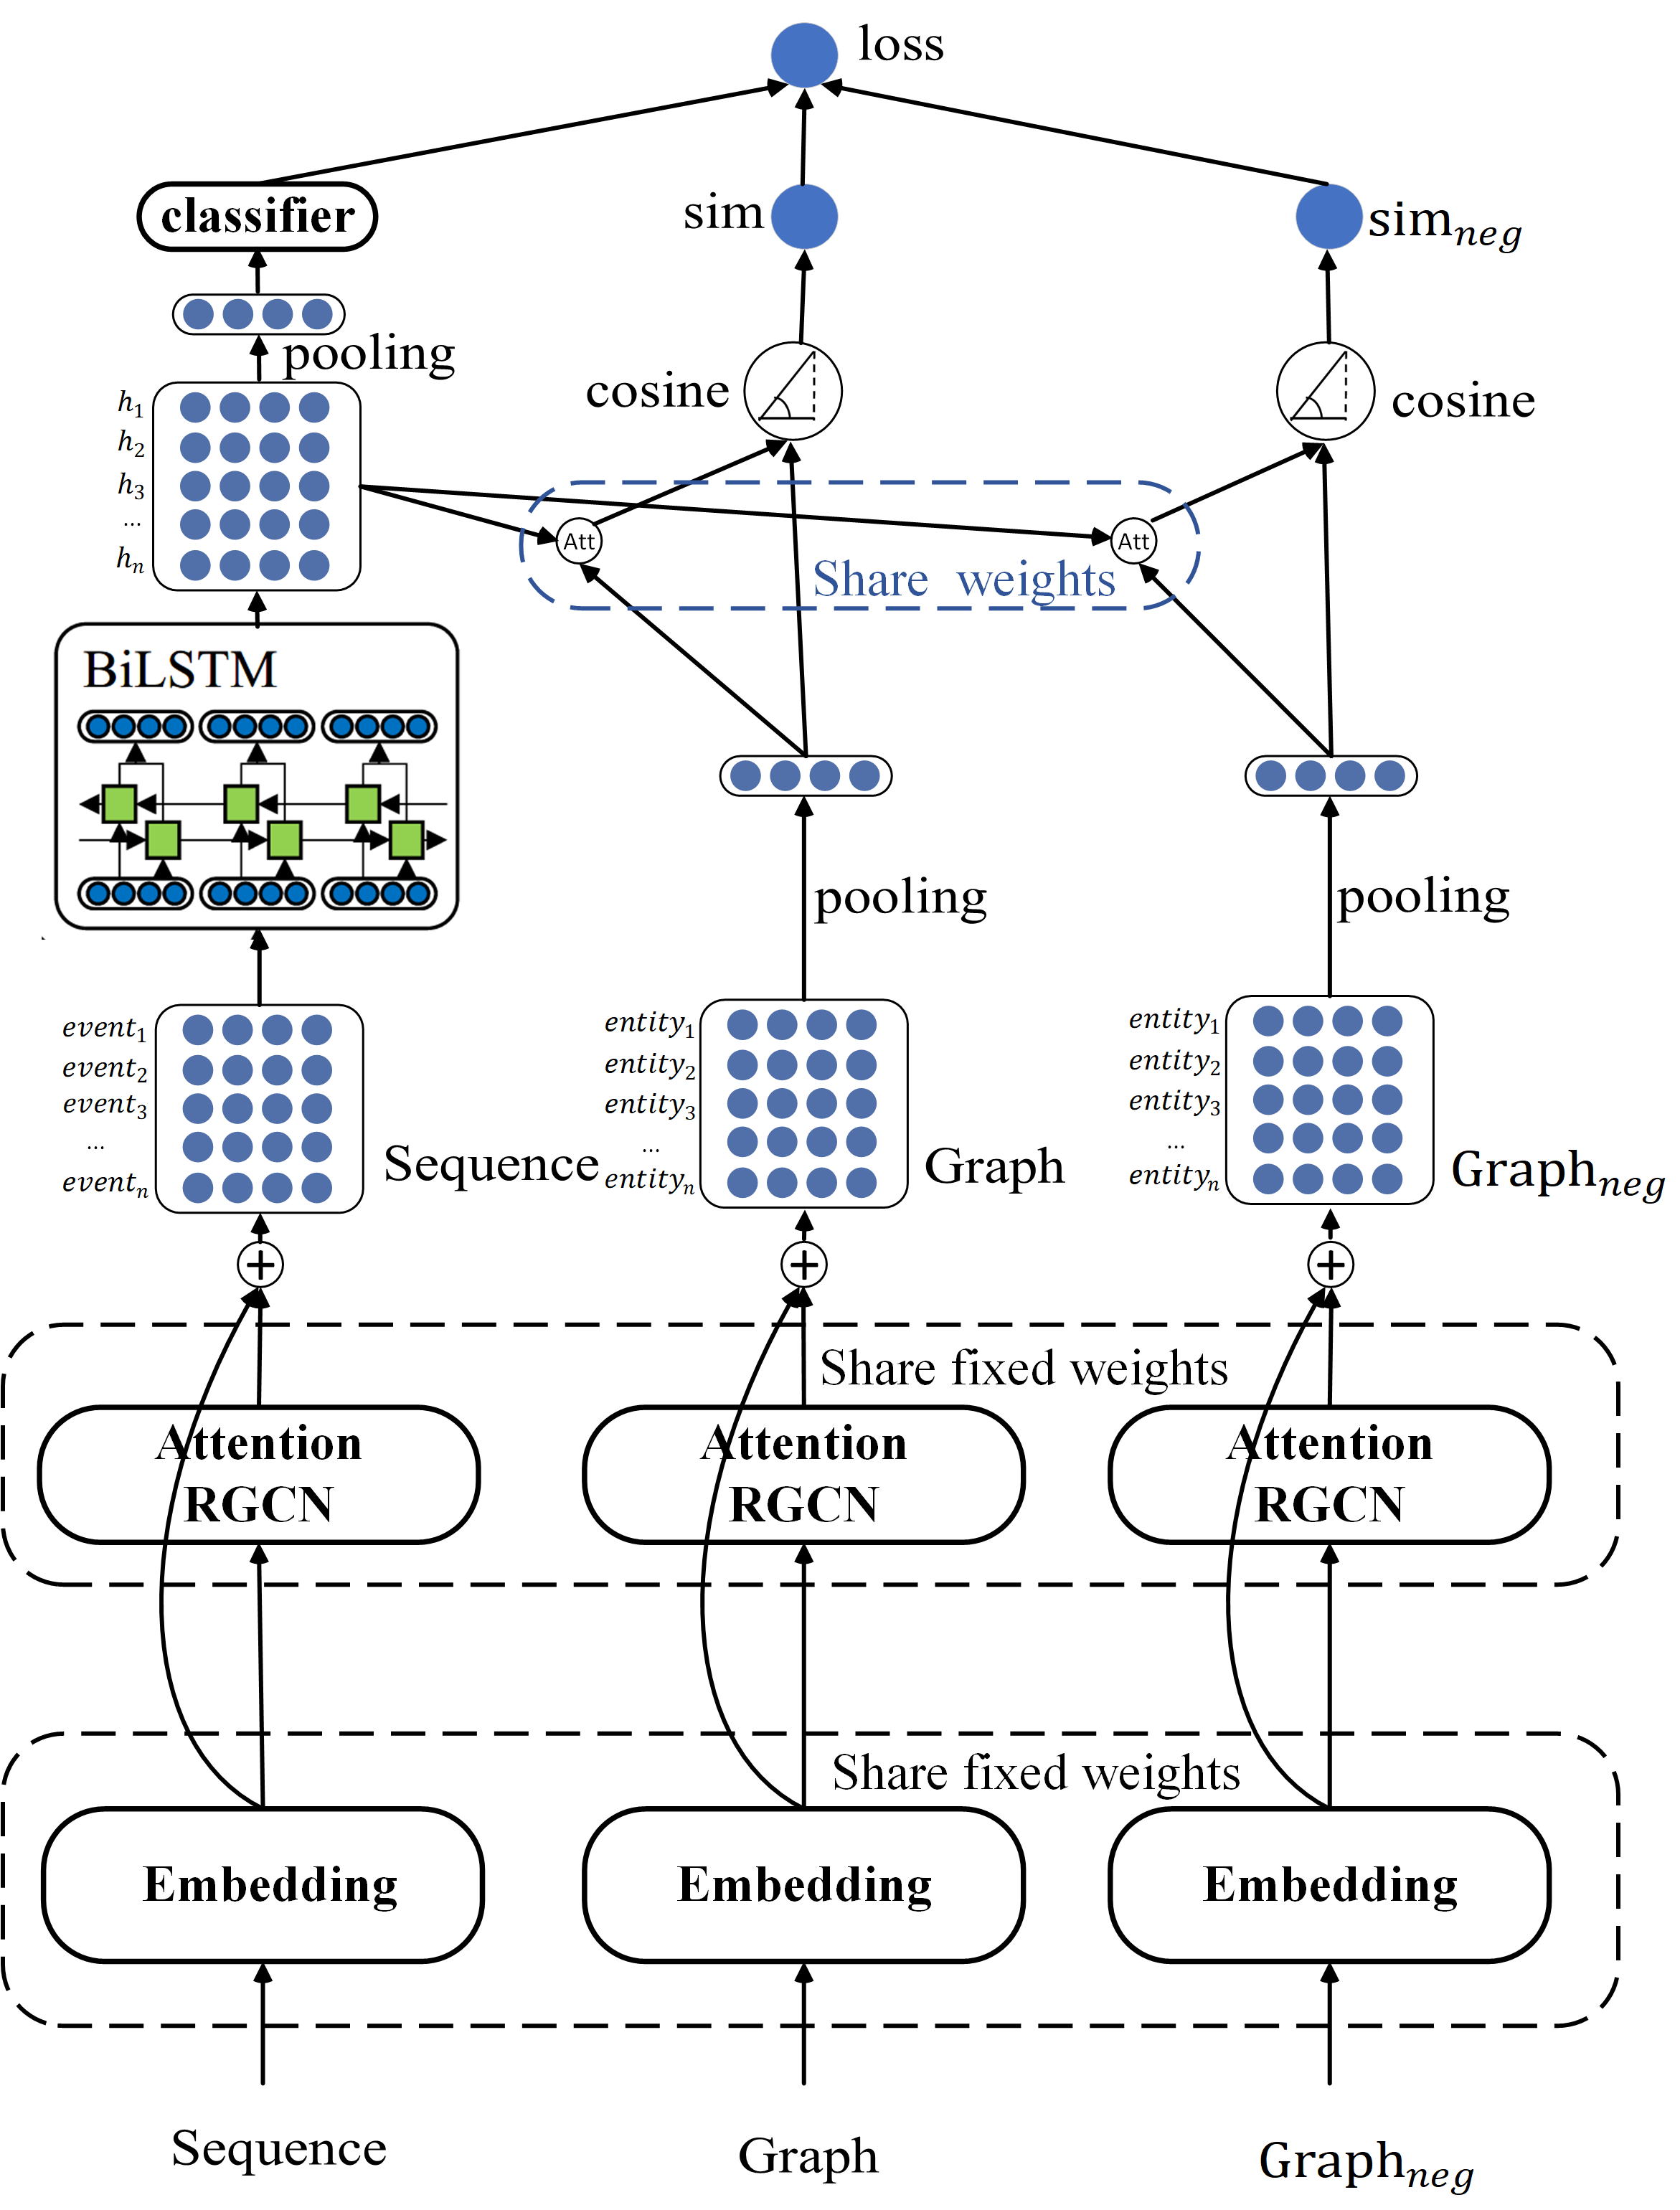
\includegraphics[width=.7\textwidth]{predict-error-model.png}
    \caption{故障预测模型\label{predict-error-model}}
\end{figure}
图\ref{predict-error-model}是引入组件-事件知识图谱的故障预测模型。其中嵌入层、Attention-RGCN使用组件-事件知识图谱表示学习模型的结构与参数,并固定不变。BiLSTM层、注意力层和分类层的参数会在后续进行学习。

嵌入层规定了实时事件序列和知识图谱的嵌入方式。图\ref{input-event-sequence}为一个实时事件序列案例,可见实时事件序列中每个事件也都对应着所在的组件,且组件之间存在着拓扑关系,只是每个组件都有其唯一标识,但对应的组件类型未发生改变,所以同样可以使用图\ref{kg-representation}中的表示学习模型,获取每个实时事件的嵌入表示向量。输入的组件-事件知识图谱则同图\ref{graph-example}所示。输入层中的embedding和Attention-RGCN均使用章节\ref{representation-paras-learn}所学到的参数并固定,实时事件序列和组件-事件知识图谱都会共享这些参数用于嵌入表示。
\begin{figure}[htbp]
    \centering
    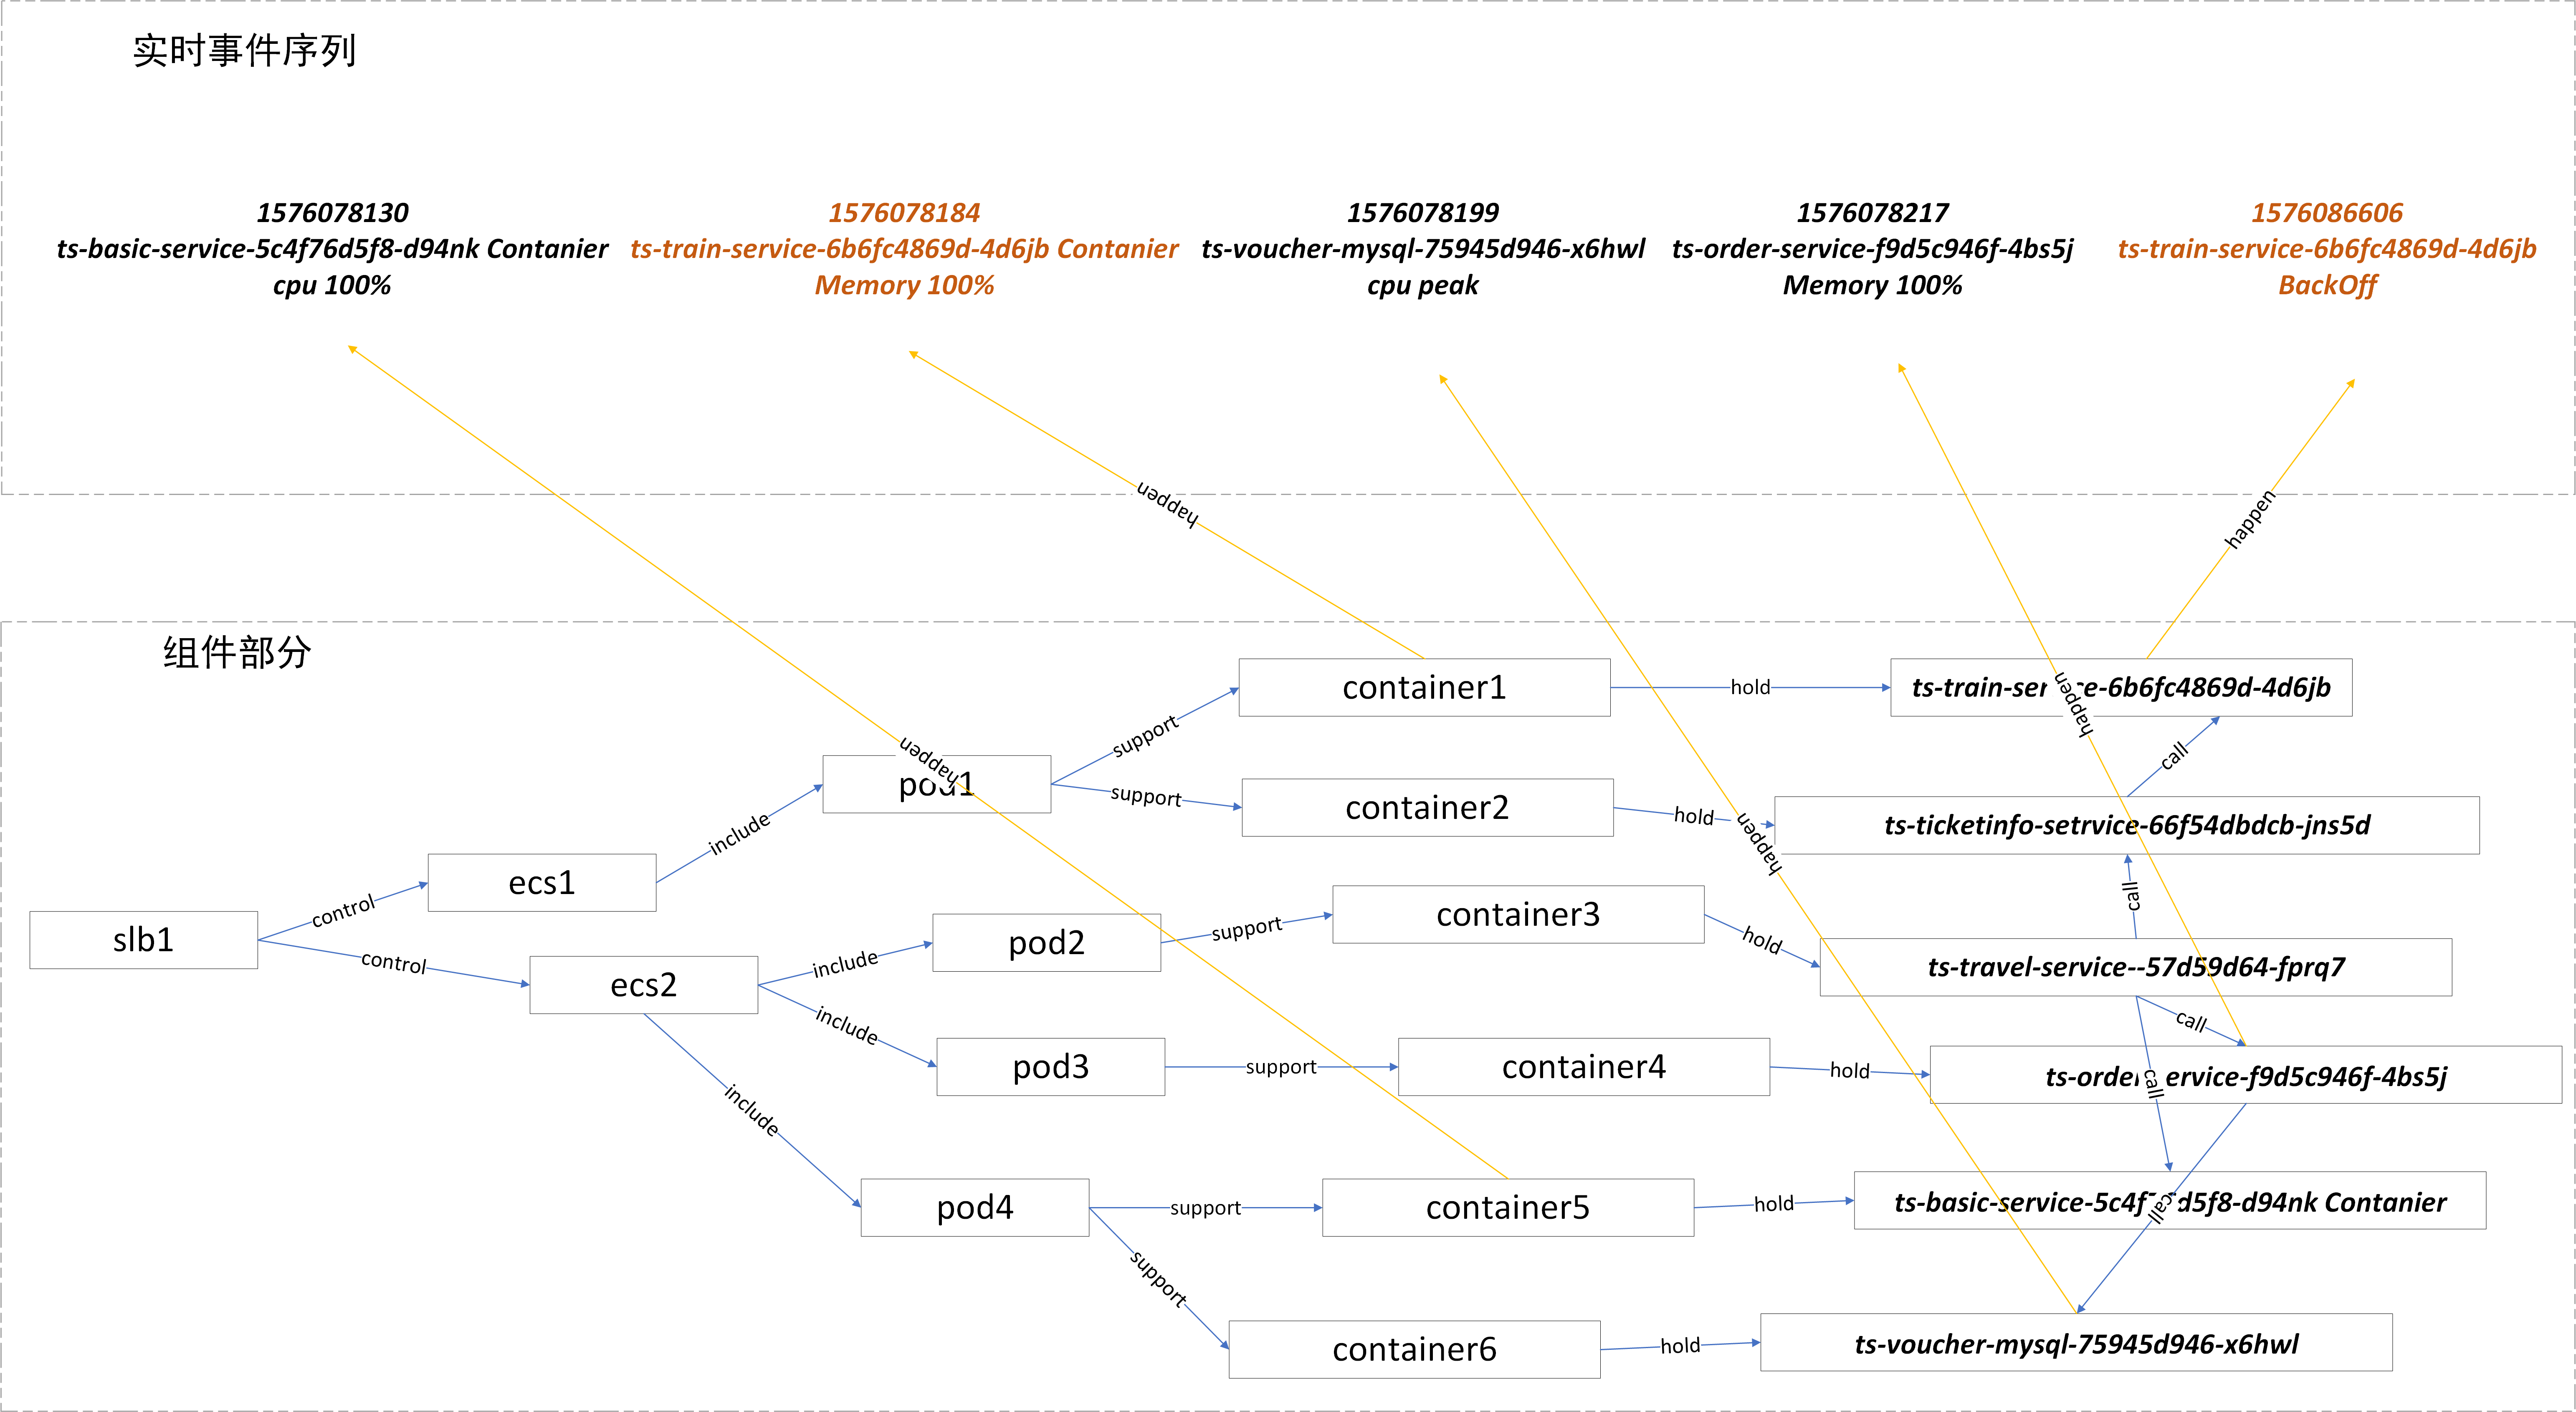
\includegraphics[width=.9\textwidth]{input-event-sequence.png}
    \caption{输入实时事件序列样例\label{input-event-sequence}}
\end{figure}

BiLSTM层用来获取实时事件序列之间的时序特征。在实时事件序列中,虽然存在着组件之间的拓扑关系,但不存在事件之间的因果关系,事件之间只存在着前后的时序信息。

在注意力层中,特定故障类型的组件-事件知识图谱会对经过BiLSTM网络得到的隐状态序列做注意力权重累加。这样的注意力计算方式可以让知识图谱选择其所关注的事件子序列,并减少了噪声事件的干扰。输入事件序列$X=\left\{x_{1}, x_{2} \ldots x_{m}\right\}$在经过嵌入层和BiLSTM网络后会得到隐向量序列$\left\{h_{1}, h_{2} \ldots h_{m}\right\}$。
\begin{equation}
    \begin{array}{l}
    e_{(h_{i} , g)} = h_{i}\mathbf{W}g\\
    \alpha_{(h_{i} , g)}=\operatorname{softmax}\left(e_{(h_{i} , g)}\right)=\frac{\exp \left(e_{(h_{i} , g)}\right)}{\sum_{j=0}^{m}  \exp \left(e_{\left(h_{j} , g\right )}\right)}\\
    h_{sequence} = \sum_{i=0}^{m}\alpha_{(h_{i} , g)}\cdot h_{i}\\
    \end{array}
    \label{sequence-hidden}
\end{equation}

如式\ref{sequence-hidden}所示,注意层会首先计算知识图谱对隐状态序列的权重$\alpha_{(. , g)}$,然后进行权重累加获取事件序列嵌入表示$h_{sequence}$。其中,$h_i$为事件$x_i$的嵌入表示,$g$为组件-事件知识图谱经过嵌入表示层后的表示向量,$\mathbf{W} \in \mathbb{R}^{d\times d}$为参数矩阵。$m$为事件序列长度,$e_{(h_{i} , g)}$为$g$对$h_{i}$的注意力值。   

输出层分为两方面,一方面会将BiLSTM网络的输出平均池化后得到的向量直接进行预测分类(有无故障),另一方面将组件-事件知识图谱的嵌入表示与注意力层权重累加得到的序列嵌入表示$h_{sequence}$做相似度计算,输出每张故障类型对应组件-事件知识图谱的匹配度评分,按得分从高至低排列,即可得到预测故障类型排列结果。

\subsection{模型训练}
模型的损失函数如式\ref{graph-sequence-predict}所示,分为两部分。在预测判别有无故障时,使用基于交叉熵的损失函数。在知识图谱相似匹配时,通过负采样用边际损失作为损失函数。
\begin{equation}
    \begin{aligned}
        \mathcal{L}=-\sum_{i=1}^{n}[Y_{i} \log \left(f\left(X_{i} \right)\right)
        +\left(1-Y_{i}\right) \log \left(1-f\left(X_{i} \right)\right)\\
+Y_{i}\cdot \max \left (0, b +\operatorname{cos} \left (h_{i},  g_{neg} \right ) - \operatorname{cos} \left (h_{i}, g \right )\right )]
    \end{aligned}
    \label{graph-sequence-predict}
\end{equation}

其中,$X_{i}$为第$i$个输入事件序列$\left\{x_{1}, x_{2} \ldots x_{m}\right\}$,$Y_{i}$为第$i$个输入事件序列有无故障的标签(0表示输入事件序列无故障,1表示输入事件序列有故障)。$h_{i}$为$X_{i}$事件序列经过如式\ref{sequence-hidden}注意力机制计算得到的隐状态嵌入表示,$g$为$X_{i}$对应故障类型的组件-事件知识图谱的嵌入表示,$g_{neg}$为负采样任意一个与$X_{i}$不匹配的组件-事件知识图谱的嵌入表示向量,$b$为损失函数的偏置超参。

根据以上损失函数计算的损失值,就可以利用梯度下降算法更新模型参数,直到模型训练完成。模型训练算法如\ref{predict-alg}所示。

\begin{algorithm}[htbp]
	\renewcommand{\algorithmicrequire}{\textbf{输入:}}
	\renewcommand{\algorithmicensure}{\textbf{输出:}}
	\caption{基于事件序列和知识图谱的故障预测模型的训练算法}
	\label{predict-alg}
	\begin{algorithmic}[1]
		\REQUIRE 带有无故障标签$Y$和具体故障类型标签的事件序列集合$X$,学习率$\alpha$,训练代数$epoch$
		\ENSURE 更新后的模型参数$\theta$
		\STATE 随机初始化模型参数$\theta$,$i \gets 0$
		\WHILE {$i<{epoch}$}
            \FORALL{$X_{i} \in X$}
                \IF {$Y_{i} == 1$}                        %条件语句
                    \STATE $g \gets$ Attention-RGCN($X_{i}$对应故障类型的组件-事件知识图谱)
                  \STATE $g_{neg} \gets$Attention-RGCN(知识库中随机一个不与$X_{i}$匹配的知识图谱)

                \ENDIF
                \STATE 如式\ref{graph-sequence-predict}计算损失值$\mathcal{L}_{\theta }\left( X_{i}\right)$
                \STATE $\theta \gets \theta - \alpha \nabla \mathcal{L}_{\theta }\left( X_{i} \right)$
            \ENDFOR
        \ENDWHILE 
		\STATE \textbf{return} $\theta$
	\end{algorithmic}  
\end{algorithm}

\subsection{模型预测}
在训练完上述基于知识图谱的故障预测模型后,该模型可用于实时的故障预测,即输入实时的异常事件序列$X$,模型会计算发生各种故障的概率,IT运维人员可根据故障预测结果及时采取防范措施。

具体计算方式为遍历故障库$failures$中每个故障$f$对应的组件-事件知识图谱$g_f$,分别与实时事件序列$X$成对输入模型$model(.)$计算匹配度评分。最后,取评分最高的故障类型$failure$作为预测结果即可,如式\ref{predict-anoma-equation}所示。
\begin{equation}
    failure = \mathop{\arg\max}\limits_{f\in failures}( model ( X, g_f)) 
    \label{predict-anoma-equation}   
\end{equation}
\section{实验与分析}
\subsection{数据集构建}
在构建组件-事件知识图谱时,表\ref{anomal-split}中的历史故障时间段数据已经被使用。本处的故障预测实验选择使用实时故障时间段数据。由于每一个故障时间段都有对应的故障类型,所以此处不需要人工标注,直接将同一故障类型的组件-事件知识图谱与事件序列视为相似,不同故障类型的知识图谱与事件序列视为不相似即可。

由于故障预测任务是根据已发生的事件序列,预测可能会出现何种故障,所以对每一个实例时间段的事件序列选择去除其最后的故障事件,只保留故障发生前的异常事件序列。另外,每个时间段的事件序列长度不一致,而BiLSTM的输入长度需要是确定的。所以,若BiLSTM的输入长度为L,对于长度小于L的事件序列填零补全至L,对于长度长于L的事件序列只保留前L个事件。

本文用于故障预测的事件序列数较少,两应用中分别有146和168条。为了扩增数据量,首先,实验将每类故障下的事件序列数按照6:2:2进行划分得到训练集、验证集、测试集;随后,遍历事件序列中每个事件,选择随机保留或去除(事件关键性越高,被保留的概率越高;反之,越低),这样遍历一次保留下来的事件序列视作随机采样得到的一条新数据;最后,对每一条事件序列随机采样9次,完成数据增强。这样随机采样生成新事件序列的方式,不仅扩充了数据,也使得模型具有了鲁棒性。模型即使利用实时产生的部分事件序列信息,也可以正确预测其可能发生的故障。最终,用于故障预测的实时事件序列数目如表\ref{event-sequence-num}所示。
% \begin{table}[htbp]
%     \centering
%     \caption{实时事件序列数}
%     \label{event-sequence-num}
%     \begin{tabular}{ccccc}
%         \midrule[1pt]
%         数据集名称        & 初始事件序列数 & 随机采样后事件序列数 & 训练集 & 测试集 \\ \midrule[1pt]
%         Train-ticket & 235     & 532     & 323 & 209 \\
%         Sock-shop    & 214     & 595     & 363 & 232 \\ \midrule[1pt]
%     \end{tabular}
% \end{table}
\begin{table}[htbp]
    \caption{实时事件序列数}
    \centering
    \label{event-sequence-num}
    \begin{tabular}{ccccc}
    \toprule[1.5pt]
    分布式应用        & \begin{tabular}[c]{@{}c@{}}初始\\ 事件序列数\end{tabular} & \begin{tabular}[c]{@{}c@{}}随机采样扩展后\\ 训练集\end{tabular} & \begin{tabular}[c]{@{}c@{}}随机采样扩展后\\ 验证集\end{tabular} & \begin{tabular}[c]{@{}c@{}}随机采样扩展后\\ 测试集\end{tabular} \\ \midrule[1.5pt]
    train-ticket & 146                                                & 870                                                   & 290                                                   & 300                                                   \\
    sock-shop    & 168                                                & 1000                                                  & 330                                                   & 350                                                   \\ \bottomrule[1.5pt]
    \end{tabular}
\end{table}

\subsection{评测指标}

本文将实时事件序列与组件-事件知识图谱进行匹配,等同于将实时事件序列按故障类型做多分类。因此,最终的评测标准以测试集中事件序列分类到组件-事件知识图谱的精确率(precision)、召回率(recall)和F1值为指标。本处多分类的精确率、召回率和F1值的计算方式为:分别计算各类别的precision、recall和F1,再取均值。

\subsection{实验方法}

在模型训练过程中,每一个事件序列除了有其对应的相似组件-事件知识图谱$G_{pos}$,还需负采样任选一个不相似的组件-事件知识图谱$G_{neg}$。模型训练目标函数为最大化两者差距,即与相似组件-事件知识图谱的匹配度评分$Sim_{pos}$要远大于与不相似的组件-事件知识图谱的匹配度评分$Sim_{neg}$。在计算测量指标时,首先将事件序列与组件-事件知识库中每个图谱都做匹配度评分计算,并按照匹配度评分降序排列。由于实验数据中类别都只有十余种,所以只在对应组件-事件知识图谱匹配度评分$Sim_{pos}$排序第一时视作分类正确。为了验证本文基于记忆网络和知识图谱的故障预测模型的性能表现,实验选用了以下几种方法对比:
\begin{itemize}[itemsep=0 pt,topsep = 0 pt,parsep =0pt,partopsep=0pt]
    \item [(1)] 
    \textbf{PREPARE}\cite{tan2012prepare}:PREPARE结合了属性值预测模型和多变量分类模型进行故障预测。属性值预测模型可以估计属性在未来时间的值分布。多变量分类模型可以计算一组估计的未来属性值映射成“正常”或“异常”状态的概率。具体实现上,该方法使用了马尔可夫模型进行属性值预测,使用了贝叶斯网络进行分类。本块实验将贝叶斯网改为多分类,以和其他方法进行对比。
    % \item [(2)]
    % \textbf{HMM}\cite{purushotham2005multi}:该方法基于隐马尔可夫模型判断当前组件是否存在会导致未来故障的错误状态来实现故障预测。本块实验在其后添加感知机和$softmax$层,将其改为多分类,以和其他方法进行对比。
    \item [(2)]
    \textbf{RNN}\cite{xu2016health}:使用循环神经网络编码事件序列,再多分类到故障类型。
    \item [(3)]
    \textbf{LSTM}\cite{cheng2018machine,du2017deeplog,das2018desh,islam2017predicting,li2020predicting}:使用长短期记忆网络编码事件序列,再多分类到故障类型。
    \item [(4)]
    \textbf{Bi-LSTM}\cite{gao2020task}:使用双向长短期记忆网络编码事件序列,再多分类到故障类型。
    \item [(5)]
    \textbf{FPKG}:本文在章节\ref{kg-pre-error}所提出的基于时序数据和知识图谱的故障预测模型。
    \item [(6)]
    \textbf{FPKG-1}:相比本文方法,去除了知识图谱对事件序列的attention机制。
    \item [(7)]
    \textbf{FPKG-2}:相比本文方法,使用RNN替换了BiLSTM。
    \item [(8)]
    \textbf{FPKG-3}:相比本文方法,使用LSTM替换了BiLSTM。

\end{itemize}

其中,PREPARE、RNN、LSTM和BiLSTM为已有代表性工作所使用的方法,在本实验中作为基线模型。为了对比各个模型,本块实验将RNN、LSTM和BiLSTM都后接了多层感知机和$softmax(.)$层进行多分类。FPKG-1用于验证知识图通过注意力机制可以选取有效信息,提升预测效果;FPKG-2用于验证在编码事件序列时BiLSTM比RNN效果更好;FPKG-3用于验证在编码事件序列时BiLSTM比LSTM效果更好。

\subsection{实验结果与分析}
\begin{table}[htbp]
    \caption{故障预测结果}
    \centering
    \label{anom-predict}
    \begin{tabular}{ccccccc}
    \toprule[1.5pt]
               &                & train-ticket   &                &                & sock-shop      &                \\
    方法         & precision      & recall         & F1             & precision      & recall         & F1             \\ \midrule[1.5pt]
    PREPARE    & 0.732          & 0.727          & 0.728          & 0.689          & 0.677          & 0.679          \\
    RNN        & 0.765          & 0.757          & 0.759          & 0.703          & 0.688          & 0.691          \\
    LSTM       & 0.789          & 0.761          & 0.772          & 0.719          & 0.691          & 0.701          \\
    BiLSTM     & 0.807          & 0.792          & 0.796          & 0.747          & 0.780          & 0.759          \\
    FPKG       & \textbf{0.939} & \textbf{0.904} & \textbf{0.918} & \textbf{0.887} & \textbf{0.848} & \textbf{0.861} \\
    FPKG-1 & 0.904          & 0.892          & 0.896          & 0.842          & 0.831          & 0.832          \\
    FPKG-2 & 0.841          & 0.815          & 0.823          & 0.787          & 0.776          & 0.782          \\
    FPKG-3 & 0.879          & 0.887          & 0.883          & 0.825          & 0.813          & 0.814          \\ \bottomrule[1.5pt]
    \end{tabular}
    \end{table}

实验记录了各个方法的精确率、召回率和F1值,结果如表\ref{anom-predict}所示。可见FPKG取得了最佳的精确率、召回率和F1值,证明了本文模型的优质性。PREPARE、RNN、LSTM和BiLSTM相比其他方法效果都较差,证明了引入知识图谱会显著提升故障预测效果。FPKG-1不如FPKG的效果,证明了注意力机制提升了故障预测效果。FPKG-3比FPKG效果差,说明了编码事件序列特征方面,LSTM不如BiLSTM。FPKG-2比FPKG-3效果更差,表明了RNN比LSTM、BiLSTM在编码事件序列时效果更差。

本块实验中,输入嵌入层和Attention-RGCN层设置为章节\ref{representation-experiment}中组件-事件知识图谱表示学习模型的结构与参数,并固定不变。本块实验效果达到最佳时,模型选用的超参数为BiLSTM层为2层、输入序列长度为1024、中间隐状态为50;序列分类器层为$100*32*2$的神经网络加$softmax(.)$层;损失函数的偏置超参$b$为0.7。

\section{本章小结}
本章主要介绍了基于实时事件序列和组件-事件知识图谱的故障预测。通过上一章的组件-事件知识图谱表示学习模型获取每个故障类型对应的组件-事件知识图谱的嵌入表示向量,然后对BiLSTM网络编码的实时事件序列隐状态进行注意力权重累加,获取事件序列嵌入表示。最后计算两个嵌入表示向量的相似度,按照相似度从高至低排序各个知识图谱即可得到预测的故障类型列表。本文的故障预测模型引入了组件-事件知识图谱,预测结果可以具体到故障类型,且具有了可解释性。另外,在数据集上的实验结果,证明了本章引入知识图谱的故障预测模型具有优越性。